\chapter{TileCal related work}
    \label{app:DetectorWork}

This appendix collects details on the Tile calorimeter (TileCal) readout electronics and detector maintenance that constituted part of this PhD Thesis work.


\section{Introduction}

TileCal is the hadronic calorimeter covering the most central region of the ATLAS experiment at the LHC.
It is a sampling calorimeter with iron plates as absorber and plastic scintillating tiles as the active material.
The readout architecture divides the detector into four partitions, two Long Barrels (LB) and two External Barrels (EB).
The detector is divided into two sides, A and C, corresponding to positive and negative pseudorapidities, respectively.
Each partition is segmented into 64 wedges, called modules, corresponding to a granularity of $\sim \unit[0.1]{rad}$ in the $\phi$-coordinate. 
Radially, each module is segmented into three layers called \emph{A}, \emph{BC} and \emph{D}, with a segmentation in $\eta$ of $0.1$ in the first two radial layers and $0.2$ in the third one. 
Figure~\ref{fig:DetectorWork_ATLAS} shows a cell division scheme of the ATLAS Tile calorimeter.
Light is conducted by fibers from the tiles to the outer part of the modules, the so-called drawer, where all photomultipliers (PMTs) and electronics are placed. 

In the readout electronics, the signals from the PMTs are first shaped using a passive shaping circuit, and then amplified in separate high (HG) and low (LG) gain branches.
The shaper, the charge injection calibration system (CIS)~\cite{Tang:2013vya}, and the gain splitting are all located on a small printed circuit board known as the 3-in-1 card~\cite{Tang:2013vya}.
In addition to the digital readout of the PMT signal, a millisecond-timescale integrator circuit is also located on the 3-in-1 card, as shown in Figure~\ref{fig:DetectorWork_integrator}.
The Tile integrator is designed to measure the PMT current during $^{137}$Cs calibrations, but also to measure the current from minimum bias proton-proton interactions at the LHC.

\begin{figure}[!ht]
\begin{center}
\mbox{
  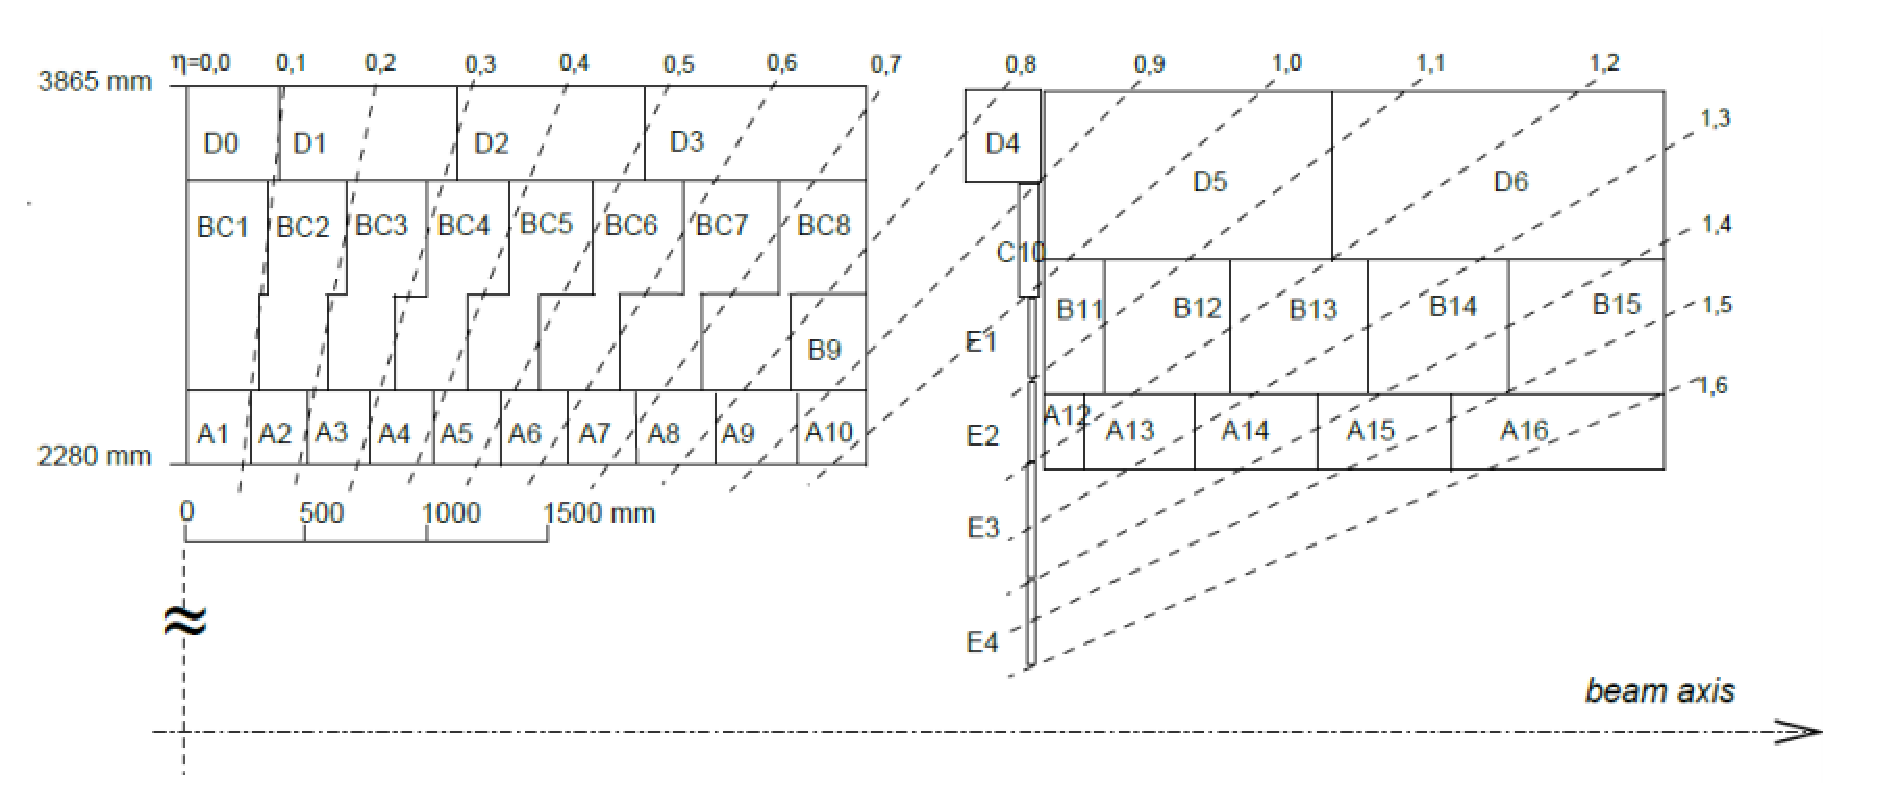
\includegraphics[width=0.995\textwidth]{Appendix_DetectorWork/Figures/ATLAS_Cells.eps}
}
\end{center}
\caption{Drawing of a half of the calorimeter divided into a barrel and an extended barrel part with the cell division scheme depicted.}
\label{fig:DetectorWork_ATLAS}
\end{figure}

\begin{figure}[!ht]
\begin{center}
\mbox{
  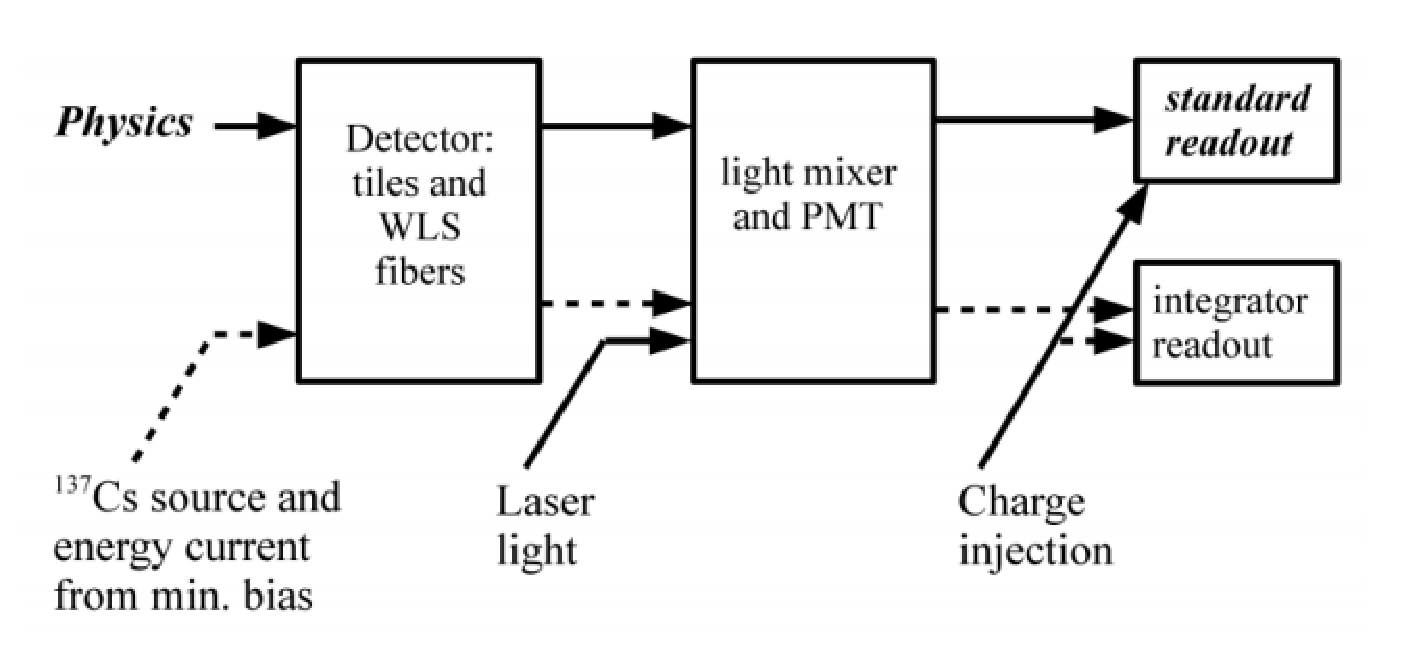
\includegraphics[width=0.795\textwidth]{Appendix_DetectorWork/Figures/ATLAS_3-in-1_Card.eps}
}
\end{center}
\caption{Flow diagram of the readout signal paths of the different TileCal calibration tools.}
\label{fig:DetectorWork_integrator}
\end{figure}



\section{Integrator}

The charge integrator is a circuit designed to measure the PMT current induced by a radioactive Cesium source as it traverses a hole through the scintillating tiles of the calorimeter~\cite{Starchenko:2002ju}, but it is also used to measure the phototube current induced by minimum bias proton-proton interactions.
This current is continuous over time and enables the integrator to monitor the response of all calorimeter cells during data-taking.
Furthermore, the integrated PMT currents are proportional to the instantaneous luminosity, and therefore can be used for luminosity measurements.

The readout of the integrated currents is performed independently for each partition.
The output of the integrator is connected to a bus on the Mother Board and sent to the Integrator card, which contains a microprocessor, a 12-bit ADC where the analogic signal is digitized, and a CANBus interface.
The data-taking proceeds as following:

\begin{enumerate}
\item The measurements of the integrated current of the PMT $i$ for each module are stored in the buffers of the CANBus\footnote{Out of the 16 buffers, 15 of them used to extract the measurement of the integrated currents, and 1 used to send commands to the CANBus. Therefore, two modules per port need to be switched after all the PMTs of the partition have been read.}.
This measurements are stored  module-by-module in the different buffers.
\item The last buffer to be filled sends a command (``dump'' command) when its memory is full, in order to retrieve the contents of all the CAN chips internal registers to the output FIFO.
\item Once the information has been retrieved, the memories are cleared and the process is repeated for the PMTs $i+1$.
\end{enumerate}

The low voltage power supplies (LVPS) adopted for the front-end electronics are located in the detector hall, in a high radiation environment. 
Each module is equipped with an independent LVPS, with a total of 256 LVPS units. 
During collisions, the Tile calorimeter faced a rate of $\sim 0.8$ LVPS trips per inverse picobarn, and a procedure to restore the data taking after each trip was adopted.
However, for the integrator readout, there was no such procedure when a trip occurred in the LVPS of a module, and therefore the integrated currents could not be retrieved for that module during the rest of the run.
If instead the trip occurred in the LVPS of the module specifically configured to send out the ``dump'' command, the loss of data was more severe, since the readout of the integrated currents for the full partition (16 modules) was stopped.

During this PhD thesis, effort has been dedicated to modify and adapt the on-line routines for the Minimum Bias data-acquisition.
To avoid the massive data loss from a full partition when a LVPS trip occurs in the module sending the ``dump'' command, the following procedure was developed and implemented:

\begin{enumerate}
\item An LVPS trip occurs.
\item\label{tripNotDump} The trip occurs in the module not sending the ``dump'' command.
\begin{enumerate}
\item No data is collected from the buffer corresponding to the tripped module, but the data flow of the partition continues.
\end{enumerate}

\item The trip occurs in the module sending the ``dump'' command.
\begin{enumerate}
\item Since the ``dump'' command cannot be sent, the data flow stops.
\item Instead, the new routine detects when the LVPS for this module has tripped. It then re-configures another module to be the one sending the ``dump'' command.
\item The data taking continues for the buffers corresponding to the non-tripped modules (back to step~\ref{tripNotDump}).
\end{enumerate}
\end{enumerate}

Finally, some effort was also dedicated to re-configure a module not sending the ``dump'' command after a trip in its LVPS.
Although the new routines worked in the spare module in the TileCal laboratory, it did not completely succeed in ATLAS due to incompatibilities with other subsystems.
In order to resolve it, more studies will be performed during Run~II.


\section{Tile Calorimeter maintenance during the LS1}

During the long shutdown 1 (LS1), tasks involving the maintenance of the front-end electronics and the consolidation of the calorimeters aiming the systematic reinforcement of the known failing problems, were performed.
The most important tasks, performed during 2013 and 2014, are listed in the following:

\begin{itemize}
\item Replace the LVPS in all the modules by a new version, more robust against trips.
\item Open and extract almost all the drawers in order to consolidate the Interface card and the flex foil connectors of the Digitizer, as shown in Figure~\ref{fig:DetectorWork_PictureATLASCavern}.
\item Perform several studies with MobiDICK~\cite{Calvet:2008zz} in order to understand the different hardware failues and to check the integrity of the TileCal super-drawers after their insertion in the TileCal modules.
\item Tile Calorimeter racks hardware replacements in ATLAS technical cavern.
\item Remove the MBTS and install 16 missing crack scintillators.
\item Hardware maintenance and upgrades of Tile Calorimeter calibration systems.
\item Control the front-end electronics spares availability.
\end{itemize}

\begin{figure}[!ht]
\begin{center}
\mbox{
  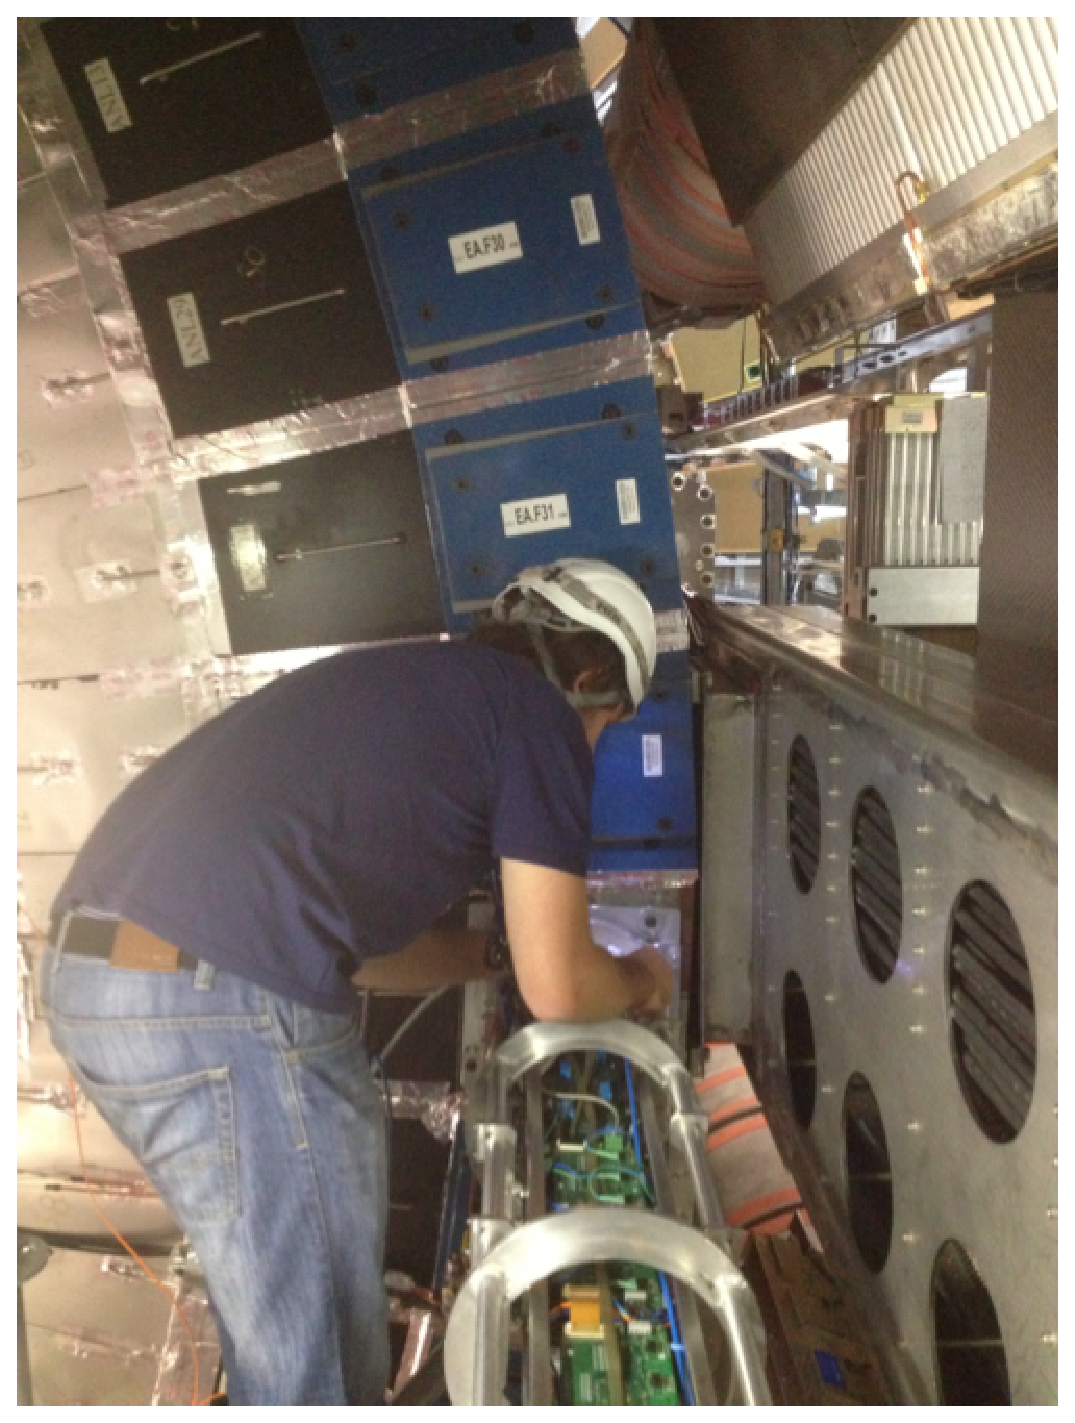
\includegraphics[width=0.495\textwidth]{Appendix_DetectorWork/Figures/PhotoATLASCavern.eps}
}
\end{center}
\caption{Roger Caminal, as part of the maintenance team, during the replacement of a moderboard connector in the ATLAS cavern.}
\label{fig:DetectorWork_PictureATLASCavern}
\end{figure}
